\documentclass[a4paper,10pt,twoside]{article}
%\usepackage{amssymb}
%\usepackage{amsthm}
\usepackage[polish]{babel}
\usepackage[utf8]{inputenc}
\usepackage[T1]{fontenc}
\usepackage{indentfirst}
\usepackage[top=2.5cm, bottom=2.5cm, left=2.5cm, right=2.5cm]{geometry}
\usepackage{graphicx}
\usepackage{amsmath}
\usepackage{booktabs}

\begin{document}

\begin{center}
\bgroup
\def\arraystretch{1.5}
\begin{tabular}{|c|c|c|c|c|c|}
	\hline
	EAIiIB & \multicolumn{2}{|c|}{Marcin Nalepa} & Rok II & \multicolumn{2}{|c|}{Grupa 5} \\
	\hline
	\multicolumn{3}{|c|}{\begin{tabular}{c}Temat: \\ Wahadło proste \end{tabular}} & 
	\multicolumn{3}{|c|}{\begin{tabular}{c}Numer ćwiczenia: \\ 0 \end{tabular}} \\
	\hline
	\begin{tabular}{@{}c@{}}Data wykonania\\07.10.2015r.\end{tabular} & \begin{tabular}{@{}c@{}}Data oddania\\15.12.2015r.\end{tabular} & 
	\begin{tabular}{c}Zwrot do\\poprawki\\\phantom{data} \end{tabular} & \begin{tabular}{c}Data oddania\\\phantom{data}\end{tabular} &
	\begin{tabular}{@{}c@{}}Data zaliczenia\\\phantom{data}\end{tabular} & \begin{tabular}{c}Ocena\\\phantom{ocena}\end{tabular} \\[4ex]
	\hline
\end{tabular}
\egroup
\end{center}

\section{Cel ćwiczenia}
Celem ćwiczenia jest wyznacznie wartości przyspieszenia grawitacyjnego Ziemi $g$ za pomocą wahadła prostego na 2 różne sposoby.

\section{Wstęp teoretyczny}
Wahadło matematyczne to punktowa masa $m$ zawieszona na nieważkiej i nierozciągliwej lince poruszająca w jednorodnym polu grawitacyjnym.
W doświadczeniu wykorzystamy bardzo dobre przybliżenie takiego układu jakim jest ciężka metalowa kulka zawieszona na nitce.

Aby znacząco uprościć obliczenia przyjmiemy $\sin\theta\approx\theta$ co jest prawdą dla małych wartości kąta $\theta$ zgodnie z
twierdzeniem Taylora. Dzięki temu ograniczamy wpływ oporu powietza na wyniki, a z uproszczonego równania ruchu wahadła
uzyskujemy następujacą zależność
\begin{equation}
T=2\pi\sqrt{\frac{l}{g}}
\end{equation}
gdzie $T$ - okres drgań, $l$ - długość nici, $g$ - przyspieszenie grawitacyjne. Po przekształceniu otrzymujemy wzór roboczy pozwalający
na wyznaczenie wartości przyspieszenia grawitacyjnego dla Ziemi
\begin{equation}
\label{eq:working_g}
g=\frac{4\pi^2l}{T^2}
\end{equation}
	
\section{Opis doświadczenia}

\begin{figure}[!htp]
\centerline{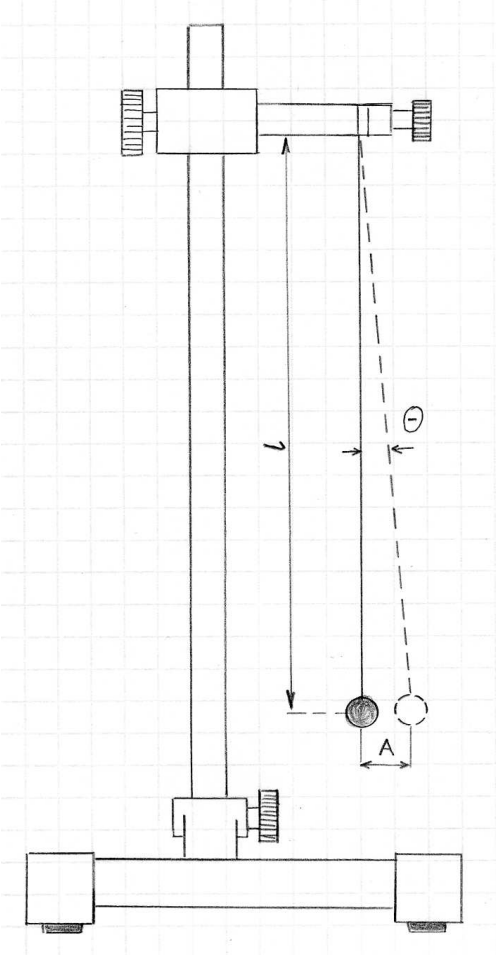
\includegraphics[scale=0.18]{wahadlo}}
\caption{Zestaw użyty w doświadczeniu}
\end{figure}
Ćwiczenie składa się z 2 części, w pierwszej dokonujemy pomiarów dla ustalonej długości wahadła, a w drugiej wyznaczamy
przyspieszenie grawitacyjne $g$ za pomocą regresji liniowej.

Na statywie zawieszono metalową kulkę na nici. Przed rozpoczęciem doświadczenia została zmierzona długość powstałego w ten sposób
wahadła za pomocą linijki. Następnie zmierzono stoperem czas trwania 10 okresów drgań wahadła. Wyniki umieszczono w tabeli.

\newpage
\section{Wyniki pomiarów}

\begin{table}[!htbp]
\caption{Stała długość wahadła $l=40,0cm$}
\centering
\def\arraystretch{1.4}
\begin{tabular}{@{}rcc@{}}
\\
\toprule
\begin{tabular}{@{}c@{}}Numer\\pomiaru\end{tabular} &
\begin{tabular}{@{}c@{}}Czas\\10 okresów [$s$]\end{tabular} &
\begin{tabular}{@{}c@{}}Czas\\1 okresu [$s$]\end{tabular}\\
\midrule
1    & 12,63 & 1,263                  \\
2    & 12,69 & 1,269                  \\
3    & 12,81 & 1,281                  \\
4    & 12,75 & 1,275                  \\ \hline
5    & 12,70 & 1,270                  \\
6    & 12,73 & 1,273                  \\
7    & 12,65 & 1,265                  \\ \bottomrule
\end{tabular}
\end{table}

\begin{table}[!htbp]
\caption{Zmienna długość wahadła}
\centering
\def\arraystretch{1.4}
\begin{tabular}{@{}rccrr@{}}
\\
\toprule
\begin{tabular}{@{}c@{}}Długość\\wahadła [$cm$]\end{tabular} &
\begin{tabular}{@{}c@{}}Średni czas\\10 okresów [$s$]\end{tabular} &
\begin{tabular}{@{}c@{}}Średni czas\\1 okresu [$s$]\end{tabular} &
\begin{tabular}{@{}c@{}}Wartość $g$\\~[$\frac{m}{s^2}$]\end{tabular} &
\begin{tabular}{@{}c@{}}Niepewność\\$u(g)$~[$\frac{m}{s^2}$]\end{tabular}\\
\midrule
16,1 & 08,07 & 0,807 & 9,75 & 0,25 \\ 
28,1 & 10,60 & 1,060 & 9,86 & 0,19 \\
34,0 & 11,66 & 1,166 & 9,86 & 0,17 \\
39,8 & 12,64 & 1,264 & 9,82 & 0,16 \\ \hline
40,0 & 12,72 & 1,272 & 9,75 & 0,16 \\
48,5 & 13,85 & 1,385 & 9,97 & 0,15 \\
54,0 & 14,72 & 1,472 & 9,83 & 0,13 \\ \bottomrule
\end{tabular}
\end{table}

\section{Opracowanie wyników}
\noindent
Ustalamy i obliczamy niepewności dla poszczególnych pomiarów:
\begin{itemize}
\item długość wahadła $u(l) = 1[mm]$
\item czas reakcji człowieka $u(T_{10}) = 10[ms] \Rightarrow u(t) = 1,0[ms]$
\end{itemize}

\subsection{Stała długość wahadła}
\noindent
Dla stałej długości wahadła stosujemy wartość średnią i odchylenie standardowe dla zestawu danych:

\begin{subequations}
\begin{equation}
\bar{g} = 9,76~\left[\frac{m}{s^2}\right]
\end{equation}
\begin{equation}
u(\bar{g}) = 0,09~\left[\frac{m}{s^2}\right]
\end{equation}
\end{subequations}
Po porównaniu z wartością tabelaryczną (Kraków $g_{krk}=9,811\left[\frac{m}{s^2}\right])$
\begin{equation}
\left| g-g_{krk} \right| = \left| 9,76-9,811 \right| = 0,051 < u(\bar{g}) = 0,090~\left[\frac{m}{s^2}\right]
\end{equation}
widać, że obliczona wartość mieści się w niepewności zwykłej.

\subsection{Zmienna długość wahadła}
\noindent
Obliczamy niepewności ze wzoru na niepewność względną
\begin{equation}
\frac{u(g)}{g} = \sqrt{\left(\frac{u(l)}{l}\right)^2 + \left(\frac{-2*u(T)}{T}\right)^2}
\end{equation}
i stąd na końcową niepewność każdego pomiaru
\begin{equation}
u(g) = g*\sqrt{\left(\frac{u(l)}{l}\right)^2 + \left(\frac{-2*u(T)}{T}\right)^2}
\end{equation}
\begin{figure}[!htp]
\centerline{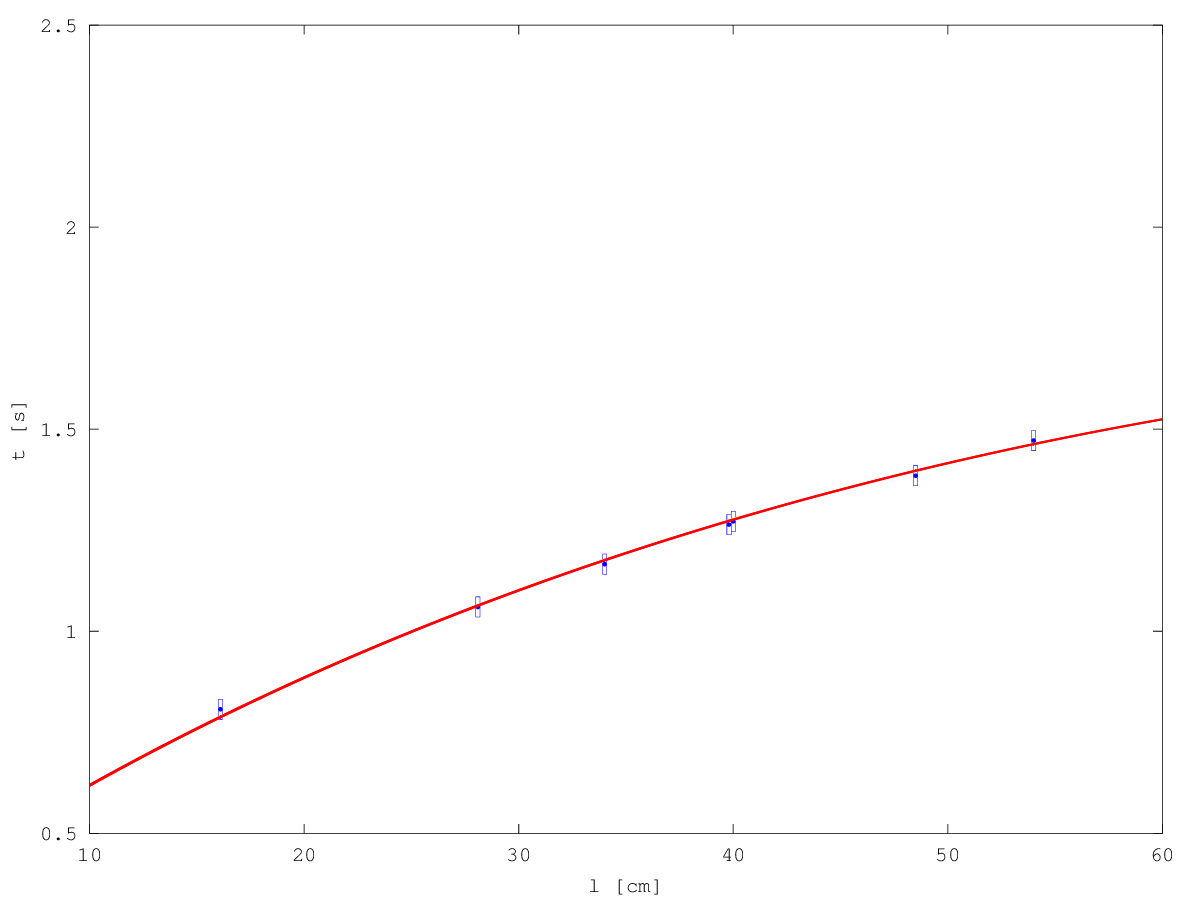
\includegraphics[scale=0.5]{plot1}}
\caption{Wykres zależnosci długości okresu od długości wahadła}
\label{fig:tl}
\end{figure}
\begin{figure}[!htp]
\centerline{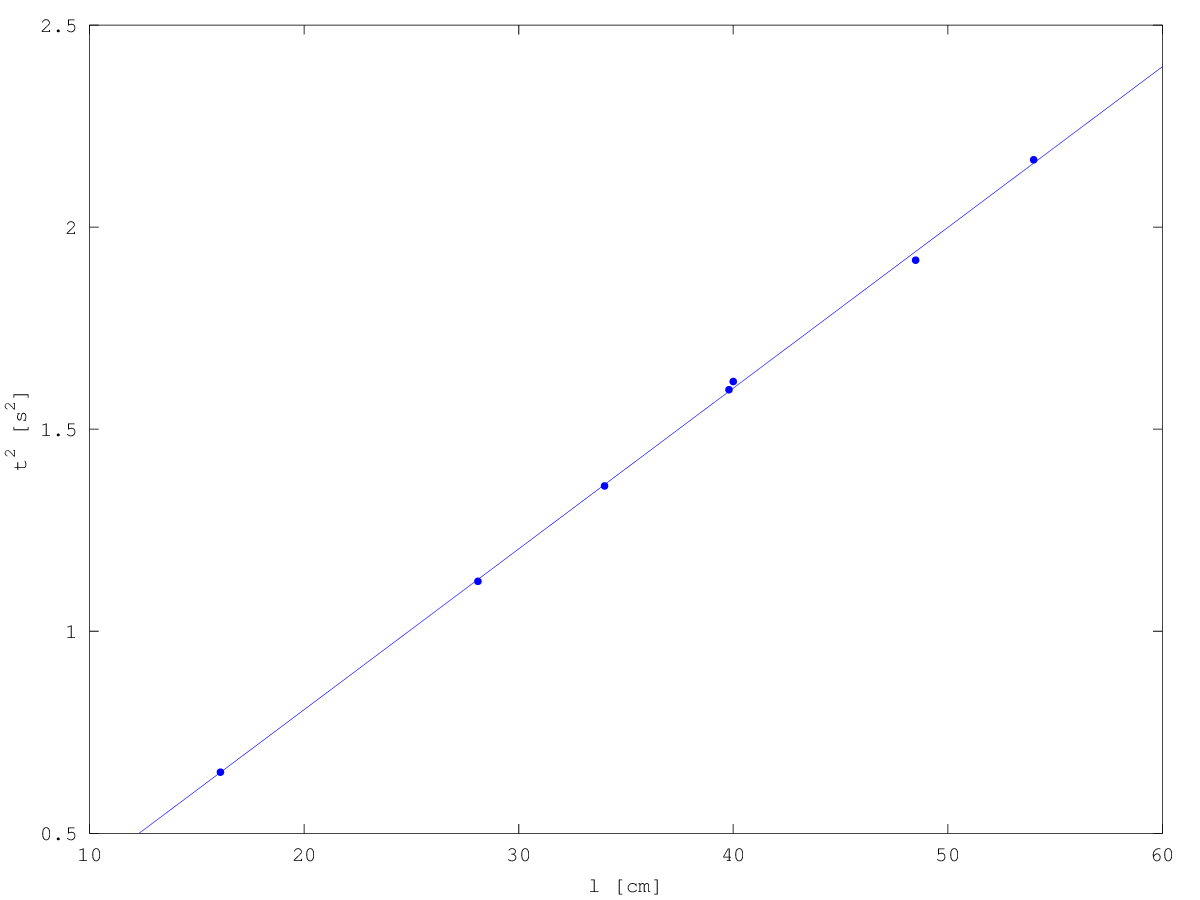
\includegraphics[scale=0.5]{plot2}}
\caption{Wykres zależnosci kwadratu długości okresu od długości wahadła}
\label{fig:ttl}
\end{figure}
\newpage
Na wykresie (\ref{fig:tl}) można zauważyć że dane nie ukłądają się do końca w lini prostej lecz delikatnie opadają.
Aby zlinearyzować wykres i mieć możliwość zastosowania regresji liniowej, podnosimy czasy okresu do kwadratu, pozbywając się
pierwiastka (\ref{fig:ttl}).

Za pomocą pakietu matematycznego wyznaczono wartość współczynnika $a$ regresji liniowej, który wykorzystamy do oblicznia
przyspieszenia grawitacyjnego $g$.
\begin{subequations}
\begin{equation}
a = 3,98
\end{equation}
\begin{equation}
u(a) = 0,04
\end{equation}
\end{subequations}
Otrzymaną wartość wstawiamy do wzoru:
\begin{subequations}
\begin{equation}
g = \frac{4\pi^2}{a} = 9,92~\left[\frac{m}{s^2}\right]
\end{equation}
\begin{equation}
u(g) = \left|-\frac{4\pi^2}{a^2}u(a)\right| = 0,10~\left[\frac{m}{s^2}\right]
\end{equation}
\end{subequations}
Porównujemy wartość z wielkością tabelaryczną
\begin{equation}
\left| g-g_{krk} \right| = \left| 9,92-9,811 \right| = 0,109 > u(g) = 0,100~\left[\frac{m}{s^2}\right]
\end{equation}
zauważamy, że obliczona wartość nie mieści się w niepewności zwykłej dlatego sprawdzamy dla niepewności rozszerzonej dla założenia $k=2$
\begin{equation}
U(g)=k*u(g)=2*0,100=0,200>0,109~\left[\frac{m}{s^2}\right]
\end{equation}
co okazuje się mieścić w spodziewanym przedziale.
\section{Podsumowanie}
Wyznaczone wartości $g$ zgadzają się ze spodziewanymi wartościami tabelarycznymi. Dokładność obliczeń w obu metodach nie różni
się znacząco, co może być spowodowane tym, że dostępnych było stosunkowo niewiele danych pomiarowych. Obie metody bardzo dobrze
przybliżają wartość przyspieszenia grawitacyjnego Ziemi.

\end{document}


























